\upaper{43}{The Constellations}
\uminitoc{The Constellation Headquarters}
\uminitoc{The Constellation Government}
\uminitoc{The Most Highs of Norlatiadek}
\uminitoc{Mount Assembly --- The Faithful of Days}
\uminitoc{The Edentia Fathers since the Lucifer Rebellion}
\uminitoc{The Gardens of God}
\uminitoc{The Univitatia}
\uminitoc{The Edentia Training Worlds}
\uminitoc{Citizenship on Edentia}
\author{Malavatia Melchizedek}
\vs p043 0:1 Urantia is commonly referred to as 606 of Satania in Norlatiadek of Nebadon, meaning the 606\ts{th} inhabited world in the local system of Satania, situated in the constellation of Norlatiadek, one of the 100 constellations of the local universe of Nebadon. Constellations being the primary divisions of a local universe, their rulers link the local systems of inhabited worlds to the central administration of the local universe on Salvington and by reflectivity to the superadministration of the Ancients of Days on Uversa.
\vs p043 0:2 \pc The government of your constellation is situated in a cluster of 771 architectural spheres, the centremost and largest of which is Edentia, the seat of the administration of the Constellation Fathers, the Most Highs of Norlatiadek. Edentia itself is approximately 100 times as large as your world. The 70 major spheres surrounding Edentia are about 10 times the size of Urantia, while the 10 satellites which revolve around each of these 70 worlds are about the size of Urantia\fnst{Note that these proportions also hold for the local system architectural spheres (see \bibref[45:0.1]{p045 0:1}). Assuming that they remain true for the spheres of the Salvington cluser, we can calculate the total surface area of all architectural worlds (cf. note at \bibref[37:10.1]{p037 10:1}): $10^4 + 70*10^2 + 70*6 + 100*(10^4 + 70*10^2 + 70*10) + 10,000*(10^4 + 7*10^2 + 7*7) = 109,277,420$. This is more than 10 times greater than the total surface of all the evolutionary worlds.}. These 771 architectural spheres are quite comparable in size to those of other constellations.\tunemarkup{pictures}{\begin{figure}[H]\centering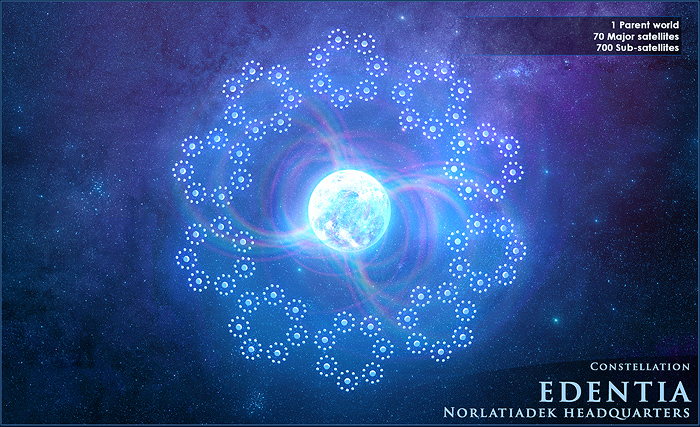
\includegraphics[angle=90,width=\tunemarkup{pgkoboaurahd}{0.7}\tunemarkup{pgnexus10}{0.9}\columnwidth]{images/EDENTIA-700.jpg}\caption{Edentia by Gary Tonge}\end{figure}}
\vs p043 0:3 \pc Edentia time reckoning and distance measurement are those of Salvington, and like the spheres of the universe capital, the constellation headquarters worlds are fully supplied with all orders of celestial intelligences. In general, these personalities are not very different from those described in connection with the universe administration.
\vs p043 0:4 The supervisor seraphim, the third order of local universe angels, are assigned to the service of the constellations. They make their headquarters on the capital spheres and minister extensively to the encircling morontia\hyp{}training worlds. In Norlatiadek the 70 major spheres, together with the 700 minor satellites, are inhabited by the univitatia, the permanent citizens of the constellation. All these architectural worlds are fully administered by the various groups of native life, for the greater part unrevealed but including the efficient spironga and the beautiful spornagia. Being the mid\hyp{}point in the morontia\hyp{}training regime, as you might suspect, the morontia life of the constellations is both typical and ideal.
\usection{The Constellation Headquarters}
\vs p043 1:1 Edentia abounds in fascinating highlands, extensive elevations of physical matter crowned with morontia life and overspread with spiritual glory, but there are no rugged mountain ranges such as appear on Urantia. There are tens of thousands of sparkling lakes and thousands upon thousands of interconnecting streams, but there are no great oceans nor torrential rivers. Only the highlands are devoid of these surface streams.
\vs p043 1:2 The water of Edentia and similar architectural spheres is no different from the water of the evolutionary planets. The water systems of such spheres are both surface and subterranean, and the moisture is in constant circulation. Edentia can be circumnavigated via these various water routes, though the chief channel of transportation is the atmosphere. Spirit beings would naturally travel above the surface of the sphere, while the morontia and material beings make use of material and semimaterial means to negotiate atmospheric passage.
\vs p043 1:3 Edentia and its associated worlds have a true atmosphere, the usual three\hyp{}gas mixture which is characteristic of such architectural creations, and which embodies the two elements of Urantian atmosphere plus that morontia gas suitable for the respiration of morontia creatures. But while this atmosphere is both material and morontial, there are no storms or hurricanes; neither is there summer nor winter. This absence of atmospheric disturbances and of seasonal variation makes it possible to embellish all outdoors on these especially created worlds.
\vs p043 1:4 The Edentia highlands are magnificent physical features, and their beauty is enhanced by the endless profusion of life which abounds throughout their length and breadth. Excepting a few rather isolated structures, these highlands contain no work of creature hands. Material and morontial ornamentations are limited to the dwelling areas. The lesser elevations are the sites of special residences and are beautifully embellished with both biologic and morontia art.
\vs p043 1:5 \pc Situated on the summit of the seventh highland range are the resurrection halls of Edentia, wherein awaken the ascending mortals of the secondary modified order of ascension. These chambers of creature reassembly are under the supervision of the Melchizedeks. The first of the receiving spheres of Edentia (like the planet Melchizedek near Salvington) also has special resurrection halls, wherein the mortals of the modified orders of ascension are reassembled.
\vs p043 1:6 The Melchizedeks also maintain two special colleges on Edentia. One, the emergency school, is devoted to the study of problems growing out of the Satania rebellion. The other, the bestowal school, is dedicated to the mastery of the new problems arising out of the fact that Michael made his final bestowal on one of the worlds of Norlatiadek. This latter college was established almost 40,000 years ago, immediately after the announcement by Michael that Urantia had been selected as the world for his final bestowal.\fnc{\ldots{}established almost \bibtextul{four} thousand years ago, immediately after\ldots{} \bibexpl{The second edition correction appears to be warranted based on a reference at \bibref[119:7.2]{p0119 7:2} in the text: “The public announcement that Michael had selected Urantia as the theatre for his final bestowal was made shortly after we learned about the default of Adam and Eve. And thus, for more than thirty-five thousand years, your world occupied a very conspicuous place in the councils of the entire universe.” The default occurred about 37,800 years ago, so “almost forty thousand” and “more than thirty-five thousand” would seem to be equally reasonable descriptions. The committee concluded that the problem here is identical in origin to that of \bibref[41:4.4]{p041 4:4} in the text: the number in question was written as a numeral in the manuscript (40,000 not forty thousand), and the error was caused by the loss of a zero before the number was formatted into words for printing.}}
\vs p043 1:7 \pc The sea of glass, the receiving area of Edentia, is near the administrative centre and is encircled by the headquarters amphitheatre. Surrounding this area are the governing centres for the 70 divisions of constellation affairs. One half of Edentia is divided into 70 triangular sections, whose boundaries converge at the headquarters buildings of their respective sectors. The remainder of this sphere is one vast natural park, the gardens of God.
\vs p043 1:8 During your periodic visits to Edentia, though the entire planet is open to your inspection, most of your time will be spent in that administrative triangle whose number corresponds to that of your current residential world. You will always be welcome as an observer in the legislative assemblies.
\vs p043 1:9 The morontia area assigned to ascending mortals resident on Edentia is located in the mid\hyp{}zone of the 35\ts{th} triangle adjoining the headquarters of the finaliters, situated in the 36\ts{th} triangle. The general headquarters of the univitatia occupies an enormous area in the mid\hyp{}region of the 34\ts{th} triangle immediately adjoining the residential reservation of the morontia citizens. From these arrangements it may be seen that provision is made for the accommodation of at least 70 major divisions of celestial life, and also that each of these 70 triangular areas is correlated with some one of the 70 major spheres of morontia training.
\vs p043 1:10 The Edentia sea of glass is one enormous circular crystal about 160\,km in circumference and about 48\,km in depth. This magnificent crystal serves as the receiving field for all transport seraphim and other beings arriving from points outside the sphere; such a sea of glass greatly facilitates the landing of transport seraphim.
\vs p043 1:11 A crystal field on this order is found on almost all architectural worlds; and it serves many purposes aside from its decorative value, being utilized for portraying superuniverse reflectivity to assembled groups and as a factor in the energy\hyp{}transformation technique for modifying the currents of space and for adapting other incoming physical\hyp{}energy streams.
\usection{The Constellation Government}
\vs p043 2:1 The constellations are the autonomous units of a local universe, each constellation being administered according to its own legislative enactments. When the courts of Nebadon sit in judgment on universe affairs, all internal matters are adjudicated in accordance with the laws prevailing in the constellation concerned. These judicial decrees of Salvington, together with the legislative enactments of the constellations, are executed by the administrators of the local systems.
\vs p043 2:2 Constellations thus function as the legislative or lawmaking units, while the local systems serve as the executive or enforcement units. The Salvington government is the supreme judicial and co\hyp{}ordinating authority.
\vs p043 2:3 \pc While the supreme judicial function rests with the central administration of a local universe, there are two subsidiary but major tribunals at the headquarters of each constellation, the Melchizedek council and the court of the Most High.
\vs p043 2:4 All judicial problems are first reviewed by the council of the Melchizedeks. Twelve of this order who have had certain requisite experience on the evolutionary planets and on the system headquarters worlds are empowered to review evidence, digest pleas, and formulate provisional verdicts, which are passed on to the court of the Most High, the reigning Constellation Father. The mortal division of this latter tribunal consists of seven judges, all of whom are ascendant mortals. The higher you ascend in the universe, the more certain you are to be judged by those of your own kind.
\vs p043 2:5 \pc The constellation legislative body is divided into three groups. The legislative program of a constellation originates in the lower house of ascenders, a group presided over by a finaliter and consisting of 1,000 representative mortals. Each system nominates 10 members to sit in this deliberative assembly. On Edentia this body is not fully recruited at the present time.
\vs p043 2:6 The mid\hyp{}chamber of legislators is composed of the seraphic hosts and their associates, other children of the local universe Mother Spirit. This group numbers 100 and is nominated by the supervising personalities who preside over the various activities of such beings as they function within the constellation.
\vs p043 2:7 The advisory or highest body of constellation legislators consists of the house of peers --- the house of the divine Sons. This corps is chosen by the Most High Fathers and numbers ten. Only Sons of special experience may serve in this upper house. This is the fact\hyp{}finding and timesaving group which very effectively serves both of the lower divisions of the legislative assembly.
\vs p043 2:8 The combined council of legislators consists of three members from each of these separate branches of the constellation deliberative assembly and is presided over by the reigning junior Most High. This group sanctions the final form of all enactments and authorizes their promulgation by the broadcasters. The approval of this supreme commission renders legislative enactments the law of the realm; their acts are final. The legislative pronouncements of Edentia constitute the fundamental law of all Norlatiadek.
\usection{The Most Highs of Norlatiadek}
\vs p043 3:1 The rulers of the constellations are of the Vorondadek order of local universe sonship. When commissioned to active duty in the universe as constellation rulers or otherwise, these Sons are known as the \bibemph{Most Highs} since they embody the highest administrative wisdom, coupled with the most farseeing and intelligent loyalty, of all the orders of the Local Universe Sons of God. Their personal integrity and their group loyalty have never been questioned; no disaffection of the Vorondadek Sons has ever occurred in Nebadon.
\vs p043 3:2 \pc At least three Vorondadek Sons are commissioned by Gabriel as the Most Highs of each of the Nebadon constellations. The presiding member of this trio is known as the \bibemph{Constellation Father} and his two associates as the \bibemph{senior Most High} and the \bibemph{junior Most High.} A Constellation Father reigns for 10,000 standard years (about 50,000 Urantia years), having previously served as junior associate and as senior associate for equal periods.
\vs p043 3:3 The Psalmist knew that Edentia was ruled by three Constellation Fathers and accordingly spoke of their abode in the plural: “There is a river, the streams whereof shall make glad the city of God, the most holy place of the tabernacles of the Most Highs\fnst{In the present Hebrew Massoretic text of Psalms~46:5(4 in Eng.), as well as all the Ancient Versions thereof which I have examined (Greek LXX, Latin Vulgate, Old Armenian, Syriac Peshitta, Aramaic Targum and Old Church Slavonic) ``the Most High'' appears in the \bibemph{singular}, not in the \bibemph{plural}.}.”
\vs p043 3:4 \pc Down through the ages there has been great confusion on Urantia regarding the various universe rulers. Many later teachers confused their vague and indefinite tribal deities with the Most High Fathers. Still later, the Hebrews merged all of these celestial rulers into a composite Deity. One teacher\fnst{This is a quote from Psalm 91:1.} understood that the Most Highs were not the Supreme Rulers, for he said, “He who dwells in the secret place of the Most High shall abide under the shadow of the Almighty.” In the Urantia records it is very difficult at times to know exactly who is referred to by the term “Most High.” But Daniel fully understood\fnst{The statement that follows is repeated \bibemph{three} times in the Book of Daniel: 4:17, 4:25 and 4:32.} these matters. He said, “The Most High rules in the kingdom of men and gives it to whomsoever he will.”
\vs p043 3:5 \pc The Constellation Fathers are little occupied with the individuals of an inhabited planet, but they are closely associated with those legislative and lawmaking functions of the constellations which so greatly concern every mortal \bibemph{race} and national \bibemph{group} of the inhabited worlds.
\vs p043 3:6 Although the constellation regime stands between you and the universe administration, as individuals you would ordinarily be little concerned with the constellation government. Your great interest would normally centre in the local system, Satania; but temporarily, Urantia is closely related to the constellation rulers because of certain system and planetary conditions growing out of the Lucifer rebellion.
\vs p043 3:7 The Edentia Most Highs seized certain phases of planetary authority on the rebellious worlds at the time of the Lucifer secession. They have continued to exercise this power, and the Ancients of Days long since confirmed this assumption of control over these wayward worlds. They will no doubt continue to exercise this assumed jurisdiction as long as Lucifer lives. Much of this authority would ordinarily, in a loyal system, be invested in the System Sovereign.
\vs p043 3:8 But there is still another way in which Urantia became peculiarly related to the Most Highs. When Michael, the Creator Son, was on his terminal bestowal mission, since the successor of Lucifer was not in full authority in the local system, all Urantia affairs which concerned the Michael bestowal were immediately supervised by the Most Highs of Norlatiadek.
\usection{Mount Assembly --- The Faithful of Days}
\vs p043 4:1 The most holy mount of assembly is the dwelling place of the Faithful of Days, the representative of the Paradise Trinity who functions on Edentia.
\vs p043 4:2 This Faithful of Days is a Trinity Son of Paradise and has been present on Edentia as the personal representative of Immanuel since the creation of the headquarters world. Ever the Faithful of Days stands at the right hand of the Constellation Fathers to counsel them, but never does he proffer advice unless it is asked for. The high Sons of Paradise never participate in the conduct of the affairs of a local universe except upon the petition of the acting rulers of such domains. But all that a Union of Days is to a Creator Son, a Faithful of Days is to the Most Highs of a constellation.
\vs p043 4:3 The residence of the Edentia Faithful of Days is the constellation centre of the Paradise system of extrauniverse communication and intelligence. These Trinity Sons, with their staffs of Havona and Paradise personalities, in liaison with the supervising Union of Days, are in direct and constant communication with their order throughout all the universes, even to Havona and Paradise.
\vs p043 4:4 The most holy mount is exquisitely beautiful and marvellously appointed, but the actual residence of the Paradise Son is modest in comparison with the central abode of the Most Highs and the surrounding 70 structures comprising the residential unit of the Vorondadek Sons. These appointments are exclusively residential; they are entirely separate from the extensive administrative headquarters buildings wherein the affairs of the constellation are transacted.
\vs p043 4:5 The residence of the Faithful of Days on Edentia is located to the north of these residences of the Most Highs and is known as the “mount of Paradise assembly.” On this consecrated highland the ascending mortals periodically assemble to hear this Son of Paradise tell of the long and intriguing journey of progressing mortals through the one billion perfection worlds of Havona and on to the indescribable delights of Paradise. And it is at these special gatherings on Mount Assembly that the morontia mortals become more fully acquainted with the various groups of personalities of origin in the central universe.
\vs p043 4:6 The traitorous Lucifer, onetime sovereign of Satania, in announcing his claims to increased jurisdiction, sought to displace all superior orders of sonship in the governmental plan of the local universe. He purposed in his heart\fnst{Isaiah~14:13-14 ``For thou hast said in thine heart, I will ascend into heaven, I will exalt my throne above the stars of God: I will sit also upon the mount of the congregation, in the sides of the north. I will ascend above the heights of the clouds; I will be like the most High.''.}, saying: “I will exalt my throne above the Sons of God; I will sit upon the mount of assembly in the north; I will be like the Most High.”
\vs p043 4:7 \pc The 100 System Sovereigns come periodically to the Edentia conclaves which deliberate on the welfare of the constellation. After the Satania rebellion the archrebels of Jerusem were wont to come up to these Edentia councils just as they had on former occasions. And there was found no way to stop this arrogant effrontery until after the bestowal of Michael on Urantia and his subsequent assumption of unlimited sovereignty throughout all Nebadon. Never, since that day, have these instigators of sin been permitted to sit in the Edentia councils of the loyal System Sovereigns.
\vs p043 4:8 That the teachers of olden times knew of these things is shown by the record\fnst{This is stated in Job~1:6 and Job~2:1.}: “And there was a day when the Sons of God came to present themselves before the Most Highs, and Satan came also and presented himself among them.” And this is a statement of fact regardless of the connection in which it chances to appear.
\vs p043 4:9 \pc Since the triumph of Christ, all Norlatiadek is being cleansed of sin and rebels. Sometime before Michael’s death in the flesh the fallen Lucifer’s associate, Satan, sought to attend such an Edentia conclave, but the solidification of sentiment against the archrebels had reached the point where the doors of sympathy were so well\hyp{}nigh universally closed that there could be found no standing ground for the Satania adversaries. When there exists no open door for the reception of evil, there exists no opportunity for the entertainment of sin. The doors of the hearts of all Edentia closed against Satan; he was unanimously rejected by the assembled System Sovereigns, and it was at this time that the Son of Man “beheld Satan fall as lightning from heaven.”
\vs p043 4:10 Since the Lucifer rebellion a new structure has been provided near the residence of the Faithful of Days. This temporary edifice is the headquarters of the Most High liaison, who functions in close touch with the Paradise Son as adviser to the constellation government in all matters respecting the policy and attitude of the order of Days toward sin and rebellion.
\usection{The Edentia Fathers since the Lucifer Rebellion}
\vs p043 5:1 The rotation of the Most Highs on Edentia was suspended at the time of the Lucifer rebellion. We now have the same rulers who were on duty at that time. We infer that no change in these rulers will be made until Lucifer and his associates are finally disposed of.
\vs p043 5:2 The present government of the constellation, however, has been expanded to include 12 Sons of the Vorondadek order. These 12 are as follows:
\vs p043 5:3 \ublistelem{1.}\bibnobreakspace The Constellation Father. The present Most High ruler of Norlatiadek is number 617,318 of the Vorondadek series of Nebadon. He saw service in many constellations throughout our local universe before taking up his Edentia responsibilities.
\vs p043 5:4 \ublistelem{2.}\bibnobreakspace The senior Most High associate.
\vs p043 5:5 \ublistelem{3.}\bibnobreakspace The junior Most High associate.
\vs p043 5:6 \ublistelem{4.}\bibnobreakspace The Most High adviser, the personal representative of Michael since his attainment of the status of a Master Son.
\vs p043 5:7 \ublistelem{5.}\bibnobreakspace The Most High executive, the personal representative of Gabriel stationed on Edentia ever since the Lucifer rebellion.
\vs p043 5:8 \ublistelem{6.}\bibnobreakspace The Most High chief of planetary observers, the director of the Vorondadek observers stationed on the isolated worlds of Satania.
\vs p043 5:9 \ublistelem{7.}\bibnobreakspace The Most High referee, the Vorondadek Son entrusted with the duty of adjusting all difficulties consequential to rebellion within the constellation.
\vs p043 5:10 \ublistelem{8.}\bibnobreakspace The Most High emergency administrator, the Vorondadek Son charged with the task of adapting the emergency enactments of the Norlatiadek legislature to the rebellion\hyp{}isolated worlds of Satania.
\vs p043 5:11 \ublistelem{9.}\bibnobreakspace The Most High mediator, the Vorondadek Son assigned to harmonize the special bestowal adjustments on Urantia with the routine administration of the constellation. The presence of certain archangel activities and numerous other irregular ministrations on Urantia, together with the special activities of the Brilliant Evening Stars on Jerusem, necessitates the functioning of this Son.
\vs p043 5:12 \ublistelem{10.}\bibnobreakspace The Most High judge\hyp{}advocate, the head of the emergency tribunal devoted to the adjustment of the special problems of Norlatiadek growing out of the confusion consequent upon the Satania rebellion.
\vs p043 5:13 \ublistelem{11.}\bibnobreakspace The Most High liaison, the Vorondadek Son attached to the Edentia rulers but commissioned as a special counsellor with the Faithful of Days regarding the best course to pursue in the management of problems pertaining to rebellion and creature disloyalty.
\vs p043 5:14 \ublistelem{12.}\bibnobreakspace The Most High director, the president of the emergency council of Edentia. All personalities assigned to Norlatiadek because of the Satania upheaval constitute the emergency council, and their presiding officer is a Vorondadek Son of extraordinary experience.
\vs p043 5:15 And this takes no account of the numerous Vorondadeks, envoys of Nebadon constellations, and others who are also resident on Edentia.
\vs p043 5:16 \pc Ever since the Lucifer rebellion the Edentia Fathers have exercised a special care over Urantia and the other isolated worlds of Satania. Long ago the prophet\fnst{The quote is from the controversial verse of Deuteronomy~32:8 which in the Hebrew ends with ``according to the number of the children of Israel'', but in the Greek LXX it ends with ``according to the number of angels of God''. Note that the present text simply omits this whole clause as irrelevant.} recognized the controlling hand of the Constellation Fathers in the affairs of nations. “When the Most High divided to the nations their inheritance, when he separated the sons of Adam, he set the bounds of the people.”
\vs p043 5:17 Every quarantined or isolated world has a Vorondadek Son acting as an observer. He does not participate in planetary administration except when ordered by the Constellation Father to intervene in the affairs of the nations. Actually it is this Most High observer who “rules in the kingdoms of men.” Urantia is one of the isolated worlds of Norlatiadek, and a Vorondadek observer has been stationed on the planet ever since the Caligastia betrayal. When Machiventa Melchizedek ministered in semimaterial form on Urantia, he paid respectful homage to the Most High observer then on duty, as it is written, “And Melchizedek, king of Salem, was the priest of the Most High.” Melchizedek revealed the relations of this Most High observer to Abraham when he said, “And blessed be the Most High, who has delivered your enemies into your hand.”
\usection{The Gardens of God}
\vs p043 6:1 The system capitals are particularly beautified with material and mineral constructions, while the universe headquarters is more reflective of spiritual glory, but the capitals of the constellations are the acme of morontia activities and living embellishments. On the constellation headquarters worlds living embellishment is more generally utilized, and it is this preponderance of life --- botanic artistry --- that causes these worlds to be called “the gardens of God.”
\vs p043 6:2 \pc About one half of Edentia is devoted to the exquisite gardens of the Most Highs, and these gardens are among the most entrancing morontia creations of the local universe. This explains why the extraordinarily beautiful places on the inhabited worlds of Norlatiadek are so often called “the garden of Eden.”
\vs p043 6:3 Centrally located in this magnificent garden is the worship shrine of the Most Highs. The Psalmist must have known something about these things, for he wrote: “Who shall ascend the hill of the Most Highs? Who shall stand in this holy place? He who has clean hands and a pure heart, who has not lifted up his soul to vanity nor sworn deceitfully.” At this shrine the Most Highs, on every tenth day of relaxation, lead all Edentia in the worshipful contemplation of God the Supreme.
\vs p043 6:4 \pc The architectural worlds enjoy 10 forms of life of the material order. On Urantia there is plant and animal life, but on such a world as Edentia there are 10 divisions of the material orders of life. Were you to view these 10 divisions of Edentia life, you would quickly classify the first three as vegetable and the last three as animal, but you would be utterly unable to comprehend the nature of the intervening four groups of prolific and fascinating forms of life.
\vs p043 6:5 Even the distinctively animal life is very different from that of the evolutionary worlds, so different that it is quite impossible to portray to mortal minds the unique character and affectionate nature of these nonspeaking creatures. There are thousands upon thousands of living creatures which your imagination could not possibly picture. The whole animal creation is of an entirely different order from the gross animal species of the evolutionary planets. But all this animal life is most intelligent and exquisitely serviceable, and all the various species are surprisingly gentle and touchingly companionable. There are no carnivorous creatures on such architectural worlds; there is nothing in all Edentia to make any living being afraid.
\vs p043 6:6 The vegetable life is also very different from that of Urantia, consisting of both material and morontia varieties. The material growths have a characteristic green colouration, but the morontia equivalents of vegetative life have a violet or orchid tinge of varying hue and reflection. Such morontia vegetation is purely an energy growth; when eaten there is no residual portion.
\vs p043 6:7 Being endowed with 10 divisions of physical life, not to mention the morontia variations, these architectural worlds provide tremendous possibilities for the biologic beautification of the landscape and of the material and the morontia structures. The celestial artisans direct the native spornagia in this extensive work of botanic decoration and biologic embellishment. Whereas your artists must resort to inert paint and lifeless marble to portray their concepts, the celestial artisans and the univitatia more frequently utilize living materials to represent their ideas and to capture their ideals.
\vs p043 6:8 If you enjoy the flowers, shrubs, and trees of Urantia, then will you feast your eyes upon the botanical beauty and the floral grandeur of the supernal gardens of Edentia. But it is beyond my powers of description to undertake to convey to the mortal mind an adequate concept of these beauties of the heavenly worlds. Truly, eye has not seen such glories as await your arrival on these worlds of the mortal\hyp{}ascension adventure.
\usection{The Univitatia}
\vs p043 7:1 Univitatia are the permanent citizens of Edentia and its associated worlds, all 770 worlds surrounding the constellation headquarters being under their supervision. These children of the Creator Son and the Creative Spirit are projected on a plane of existence in between the material and the spiritual, but they are not morontia creatures. The natives of each of the 70 major spheres of Edentia possess different visible forms, and the morontia mortals have their morontia forms attuned to correspond with the ascending scale of the univitatia each time they change residence from one Edentia sphere to another as they pass successively from world number 1 to world number 70.
\vs p043 7:2 Spiritually, the univitatia are alike; intellectually, they vary as do mortals; in form, they much resemble the morontia state of existence, and they are created to function in 70 diverse orders of personality. Each of these orders of univitatia exhibits 10 major variations of intellectual activity, and each of these varying intellectual types presides over the special training and cultural schools of progressive occupational or practical socialization on some one of the 10 satellites which swing around each of the major Edentia worlds.
\vs p043 7:3 These 700 minor worlds are technical spheres of practical education in the working of the entire local universe and are open to all classes of intelligent beings. These training schools of special skill and technical knowledge are not conducted exclusively for ascending mortals, although morontia students constitute by far the largest group of all those who attend these courses of training. When you are received on any one of the 70 major worlds of social culture, you are immediately given clearance for each of the 10 surrounding satellites.
\vs p043 7:4 In the various courtesy colonies, ascending morontia mortals predominate among the reversion directors, but the univitatia represent the largest group associated with the Nebadon corps of celestial artisans. In all Orvonton no extra\hyp{}Havona beings excepting the Uversa abandonters can equal the univitatia in artistic skill, social adaptability, and co\hyp{}ordinating cleverness.
\vs p043 7:5 These citizens of the constellation are not actually members of the artisan corps, but they freely work with all groups and contribute much to making the constellation worlds the chief spheres for the realization of the magnificent artistic possibilities of transition culture. They do not function beyond the confines of the constellation headquarters worlds.
\usection{The Edentia Training Worlds}
\vs p043 8:1 The physical endowment of Edentia and its surrounding spheres is well\hyp{}nigh perfect; they could hardly equal the spiritual grandeur of the spheres of Salvington, but they far surpass the glories of the training worlds of Jerusem. All these Edentia spheres are energized directly by the universal space currents, and their enormous power systems, both material and morontial, are expertly supervised and distributed by the constellation centres, assisted by a competent corps of Master Physical Controllers and Morontia Power Supervisors.
\vs p043 8:2 The time spent on the 70 training worlds of transition morontia culture associated with the Edentia age of mortal ascension, is the most settled period in an ascending mortal’s career up to the status of a finaliter; this is really the typical morontia life. While you are re\hyp{}keyed each time you pass from one major cultural world to another, you retain the same morontia body, and there are no periods of personality unconsciousness.\fnc{While you are \bibtextul{rekeyed} each time\ldots{} \bibexpl{The only other occurrence of re-keyed is in hyphenated form \bibref[48:2.21]{p048 2:21} in the text. Words formed with the “re-” prefix, fall under the same general Chicago Manual of Style rule, but this instance is covered by an exception: “a) When the first vowel of the added word would\ldots{}suggest mispronunciation, the hyphen is retained.” In this case, the un-hyphenated form appears to indicate that the first syllable is pronounced with a short e, causing the reader to stumble. Insertion of the hyphen resolves the problem.}}
\vs p043 8:3 Your sojourn on Edentia and its associated spheres will be chiefly occupied with the mastery of group ethics, the secret of pleasant and profitable interrelationship between the various universe and superuniverse orders of intelligent personalities.
\vs p043 8:4 On the mansion worlds you completed the unification of the evolving mortal personality; on the system capital you attained Jerusem citizenship and achieved the willingness to submit the self to the disciplines of group activities and co\hyp{}ordinated undertakings; but now on the constellation training worlds you are to achieve the real socialization of your evolving morontia personality. This supernal cultural acquirement consists in learning how to:
\vs p043 8:5 \ublistelem{1.}\bibnobreakspace Live happily and work effectively with 10 diverse fellow morontians, while 10 such groups are associated in companies of 100 and then federated in corps of 1,000.
\vs p043 8:6 \ublistelem{2.}\bibnobreakspace Abide joyfully and co\hyp{}operate heartily with 10 univitatia, who, though similar intellectually to morontia beings, are very different in every other way. And then must you function with this group of 10 as it co\hyp{}ordinates with 10 other families, which are in turn confederated into a corps of 1,000 univitatia.
\vs p043 8:7 \ublistelem{3.}\bibnobreakspace Achieve simultaneous adjustment to both fellow morontians and these host univitatia. Acquire the ability voluntarily and effectively to co\hyp{}operate with your own order of beings in close working association with a somewhat dissimilar group of intelligent creatures.
\vs p043 8:8 \ublistelem{4.}\bibnobreakspace While thus socially functioning with beings like and unlike yourself, achieve intellectual harmony with, and make vocational adjustment to, both groups of associates.
\vs p043 8:9 \ublistelem{5.}\bibnobreakspace While attaining satisfactory socialization of the personality on intellectual and vocational levels, further perfect the ability to live in intimate contact with similar and slightly dissimilar beings with ever\hyp{}lessening irritability and ever\hyp{}diminishing resentment. The reversion directors contribute much to this latter attainment through their group\hyp{}play activities.
\vs p043 8:10 \ublistelem{6.}\bibnobreakspace Adjust all of these various socialization techniques to the furtherance of the progressive co\hyp{}ordination of the Paradise\hyp{}ascension career; augment universe insight by enhancing the ability to grasp the eternal goal\hyp{}meanings concealed within these seemingly insignificant time\hyp{}space activities.
\vs p043 8:11 \ublistelem{7.}\bibnobreakspace And then, climax all of these procedures of multisocialization with the concurrent enhancement of spiritual insight as it pertains to the augmentation of all phases of personal endowment through group spiritual association and morontia co\hyp{}ordination. Intellectually, socially, and spiritually two moral creatures do not merely double their personal potentials of universe achievement by partnership technique; they more nearly quadruple their attainment and accomplishment possibilities.
\vs p043 8:12 \pc We have portrayed Edentia socialization as an association of a morontia mortal with a univitatia family group consisting of 10 intellectually dissimilar individuals concomitant with a similar association with 10 fellow morontians. But on the first seven major worlds only 1 ascending mortal lives with 10 univitatia. On the second group of seven major worlds 2 mortals abide with each native group of 10, and so on up until, on the last group of seven major spheres, 10 morontia beings are domiciled with 10 univitatia. As you learn how better to socialize with the univitatia, you will practise such improved ethics in your relations with your fellow morontia progressors.
\vs p043 8:13 As ascending mortals you will enjoy your sojourn on the progress worlds of Edentia, but you will not experience that personal thrill of satisfaction which characterizes your initial contact with universe affairs on the system headquarters or your farewell touch with these realities on the final worlds of the universe capital.
\usection{Citizenship on Edentia}
\vs p043 9:1 After graduation from world number 70, ascending mortals take up residence on Edentia. Ascenders now, for the first time, attend the “assemblies of Paradise” and hear the story of their far\hyp{}flung career as it is depicted by the Faithful of Days, the first of the Supreme Trinity\hyp{}origin Personalities they have met.
\vs p043 9:2 \pc This entire sojourn on the constellation training worlds, culminating in Edentia citizenship, is a period of true and heavenly bliss for the morontia progressors. Throughout your sojourn on the system worlds you were evolving from a near\hyp{}animal to a morontia creature; you were more material than spiritual. On the Salvington spheres you will be evolving from a morontia being to the status of a true spirit; you will be more spiritual than material. But on Edentia, ascenders are midway between their former and their future estates, midway in their passage from evolutionary animal to ascending spirit. During your whole stay on Edentia and its worlds you are “as the angels”; you are constantly progressing but all the while maintaining a general and a typical morontia status.
\vs p043 9:3 This constellation sojourn of an ascending mortal is the most uniform and stabilized epoch in the entire career of morontia progression. This experience constitutes the prespirit socialization training of the ascenders. It is analogous to the prefinaliter spiritual experience of Havona and to the preabsonite training on Paradise.
\vs p043 9:4 \pc Ascending mortals on Edentia are chiefly occupied with the assignments on the 70 progressive univitatia worlds. They also serve in varied capacities on Edentia itself, mainly in conjunction with the constellation program concerned with group, racial, national, and planetary welfare. The Most Highs are not so much engaged in fostering individual advancement on the inhabited worlds; they rule in the kingdoms of men rather than in the hearts of individuals.
\vs p043 9:5 And on that day when you are prepared to leave Edentia for the Salvington career, you will pause and look back on one of the most beautiful and most refreshing of all your epochs of training this side of Paradise. But the glory of it all augments as you ascend inward and achieve increased capacity for enlarged appreciation of divine meanings and spiritual values.
\vsetoff
\vs p043 9:6 [Sponsored by Malavatia Melchizedek.]
\quizlink
